%!TEX root = featurecalc.tex
\subsection{Radial Line Length (RLL)}
\label{ssec:methodology:rll}

HCA is a coarse summary of the ROI characteristics. Different sample may have a similar area but dramatically different shape or contour of that area. To describe this shape characteristic, we need more elements to represent the ROI. The Radial Line Length (RLL) is then introduced for this purpose.

First, we calculate the centroid of the first level  $L^1$, thereafter we treat it as the reference point $P_{ref}$ for all levels. Then, from $P_{ref}$ we draw M radial lines which intersect with the contour of every level. RLL is defined as the distance from the intersection point to $P_{ref}$. The radial lines are distributed at equal angles. We record these radial lines from the inner layers to the outer layers starting with the horizontal direction by an $M$ by $N$ dimensional vector
\begin{equation}
R_i, i=1,2,\dots,M\times N
\end{equation}
where $M$ is the number of radial lines and $N$ is the number of cross-sections.

Figure ~\ref{fig:methodology:rll8} through ~\ref{fig:methodology:rll64} show some examples of RLL. This is a more detailed description than HCA as it takes the shape of each area into consideration.

\begin{figure}[htb]
\centering
\subfigure[$M=8$]{
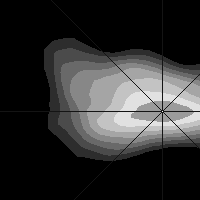
\includegraphics[width=0.4\textwidth]{ch-methodology/figures/rll8}
\label{fig:methodology:rll8}
}\hspace{0.15\linewidth}
\subfigure[$M=16$]{
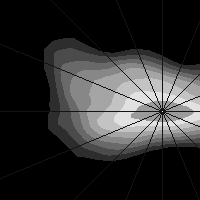
\includegraphics[width=0.4\textwidth]{ch-methodology/figures/rll16}
\label{fig:methodology:rll16}
}\\
\subfigure[$M=32$]{
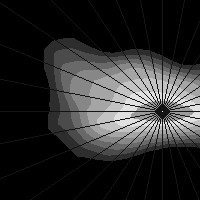
\includegraphics[width=0.4\textwidth]{ch-methodology/figures/rll32}
\label{fig:methodology:rll32}
}\hspace{0.15\linewidth}
\subfigure[$M=64$]{
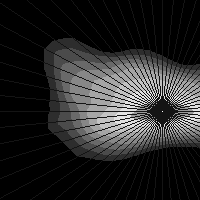
\includegraphics[width=0.4\textwidth]{ch-methodology/figures/rll64}
\label{fig:methodology:rll64}
}
\caption{$M=8,16,32,64$ radial lines starting from the reference point}
\label{fig:methodology:rllm}
\end{figure}
